\begin{frame}[c]{In a Nutshell}

\includegraphics[width=0.99\textwidth]{images/aad_comic}

\end{frame}
%----------------------------------------------------------------------
%----------------------------------------------------------------------
\begin{frame}[c]{}

\huge
\centering
What are your expectations for the course?

\bigskip

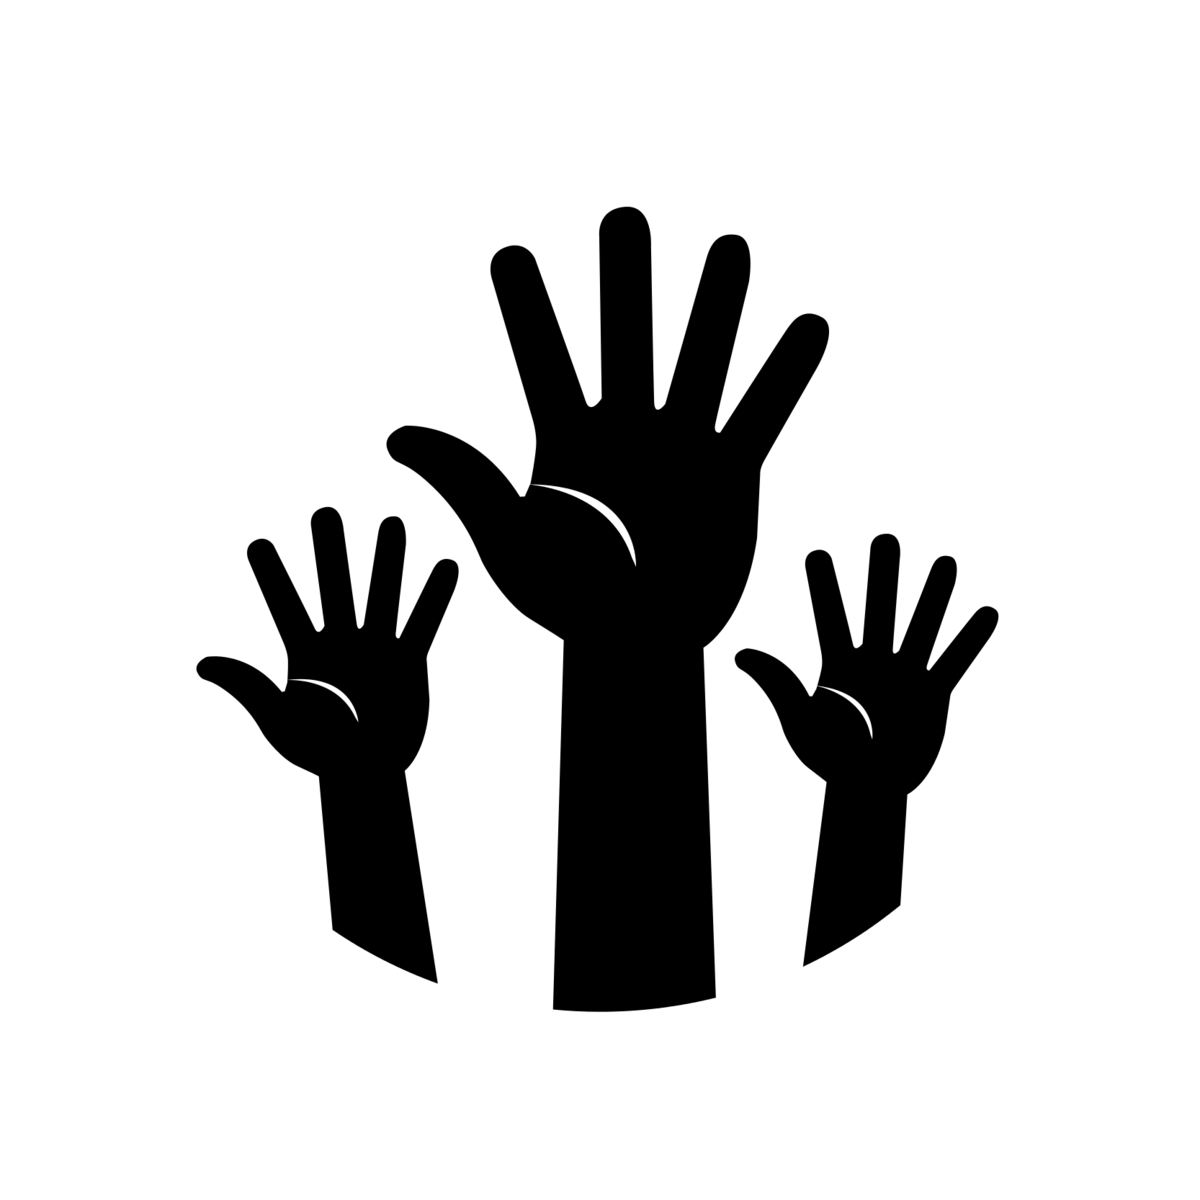
\includegraphics[scale=0.1]{images/hands.png}

\end{frame}
%----------------------------------------------------------------------
\begin{frame}[c]{}

\centering
\huge
Lecture 1:\\
Overview and Motivation
\end{frame}
%----------------------------------------------------------------------
%----------------------------------------------------------------------
\begin{frame}[c]{Overview}

What do we learn today?

\begin{itemize}
  \item What is algorithm design?
  \item Applications of machine learning and optimization\\ in algorithm design:
  \begin{itemize}
  	\item Configuration
	\item Selection 
	%\item Programming by optimization
  \end{itemize} 
  \item Why is (combinatorial) optimization important?
  \item Why is machine learning important?
  \item Real-world applications
%  \item Challenges in implementing a well-performing solver
%  \item Gap between theory and practice
  \item Organization of the course
\end{itemize}

\end{frame}
%-----------------------------------------------------------------------
%----------------------------------------------------------------------
\begin{frame}[c]{Algorithms and Applications?}

\includegraphics[width=1.\textwidth]{images/applications_add.png}

\end{frame}
%-----------------------------------------------------------------------
%----------------------------------------------------------------------
\begin{frame}[c]{Algorithm Design?}

\centering
\includegraphics[width=1.\textwidth]{images/aad}

\end{frame}
%-----------------------------------------------------------------------
%----------------------------------------------------------------------
\begin{frame}[c]{Algorithm Design?}

{\large
What is algorithm design?}

\bigskip
\pause

\begin{itemize}
  \item Software architecture
  %\item Programming language
  \item Low-level functions (e.g., merge sort vs. quick sort)
  \item Data structures
  \item Randomization
  \medskip
  \pause
  \item \alert{Magic Constants vs. Parameters}
  \item \alert{Algorithm A vs. Algorithm B}
\end{itemize}

\end{frame}
%-----------------------------------------------------------------------
%----------------------------------------------------------------------
\begin{frame}[c]{Algorithm Design?}

\centering
\includegraphics[width=1.\textwidth]{images/aad}

\end{frame}
%-----------------------------------------------------------------------
%----------------------------------------------------------------------
\begin{frame}[c]{Importance of Algorithm Design}

{\large
What are possible performance metrics?
}

\bigskip
\bigskip

\only<1-1>{
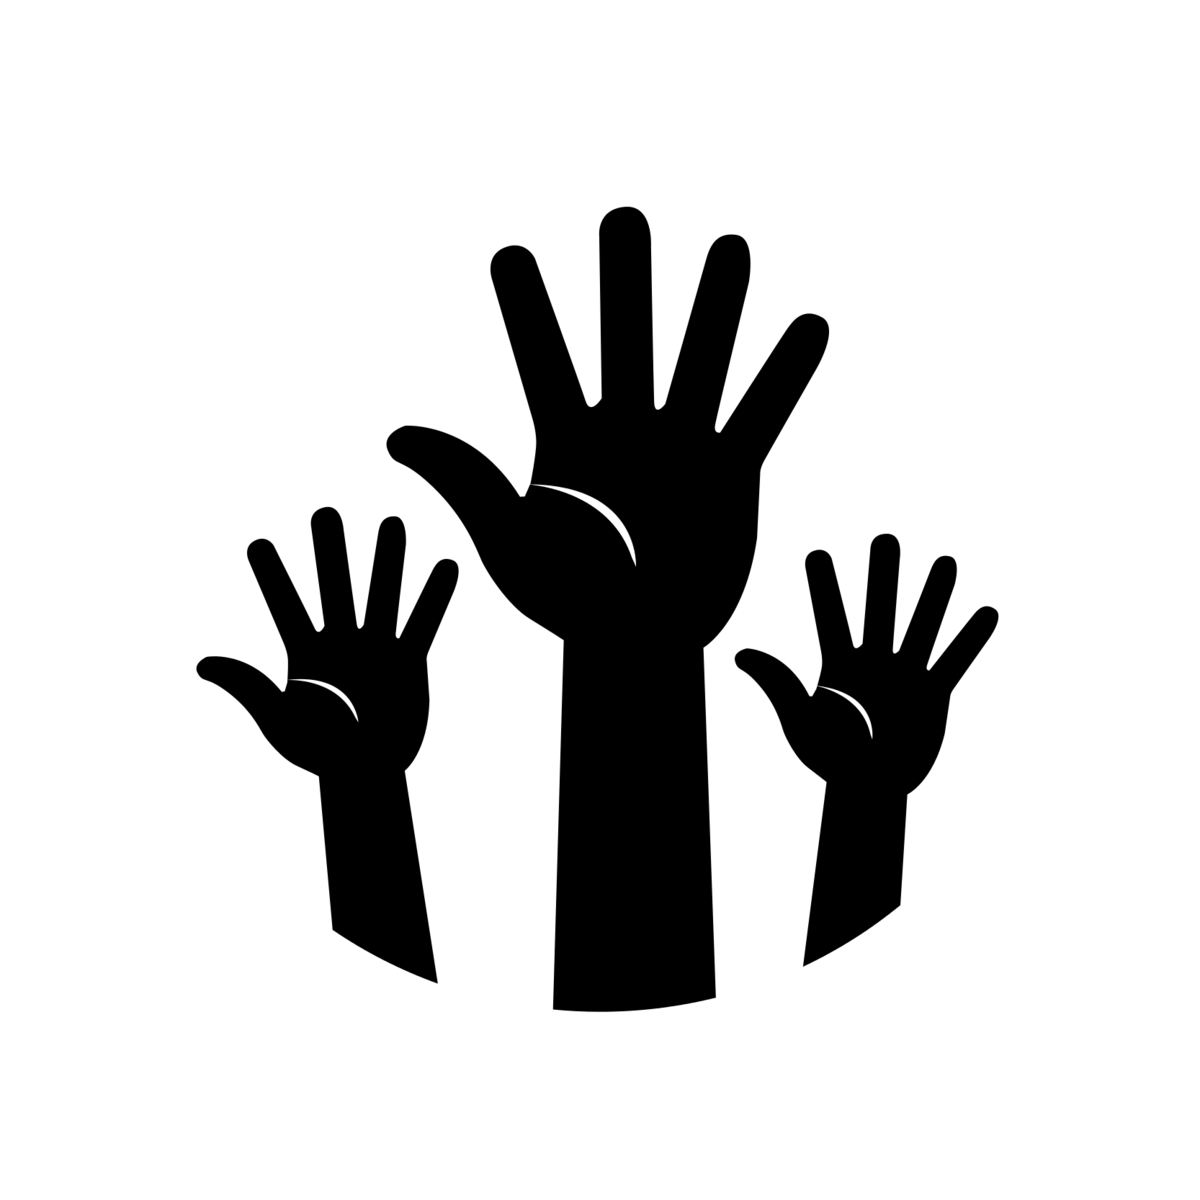
\includegraphics[scale=0.1]{images/hands.png}
}

\only<2->{
\begin{itemize}
  \item \alert{Performance}
  \pause
  \smallskip
  \begin{itemize}
    \item Runtime
    \item Memory consumption
    \item Solution quality
    \item Error
    \item \ldots
  \end{itemize}
  \medskip
  \item not covered in this course:
  \begin{itemize}
	\item Maintainability
  	\item Security
  \end{itemize}
\end{itemize}
}

\only<3->{
\alert{Note: I will use ``performance metric'' and ``cost metric'' as synonyms.}
}

\end{frame}
%-----------------------------------------------------------------------
%----------------------------------------------------------------------
\begin{frame}[c]{Algorithm Design?}

\centering
\includegraphics[width=1.\textwidth]{images/aad}

\end{frame}
%-----------------------------------------------------------------------
%----------------------------------------------------------------------
\begin{frame}[c]{Instances/Problems/Tasks/Inputs?}

Many synonums for the same concept: instances, problem, tasks, inputs, workload \ldots

Examples:

\begin{itemize}
  \item SAT instance
  \item AI planning instance
  \item logistic problem
  \item machine learning dataset
  \item data in a database
  \item \ldots
\end{itemize}


\end{frame}
%-----------------------------------------------------------------------
%----------------------------------------------------------------------
\begin{frame}[c]{Generalization of Performance}

The dark ages
\begin{enumerate}
  \item Student tweaks the parameters manually on \alert{1} problem until it works
  \item Supervisor may not even know about the tuning
  \item Results get published without acknowledging the tuning
  \item Of course, the approach \alert{does not generalize}  
\end{enumerate}

\medskip
\pause

A step further
\begin{itemize}
  \item Optimize parameters on a \alert{training set} 
  \item Evaluate generalization on a \alert{test set} 
\end{itemize}

\medskip
\pause

What you should do: avoid ``\alert{peeking}'' at the test set
\begin{itemize}
  \item Put test set into a vault (i.e., never look at it)
  \item Split training set again into \alert{training} and \alert{validation} set
  \item Only use test set in the very end to generate results\\ for publication  
\end{itemize}

\end{frame}
%-----------------------------------------------------------------------
%----------------------------------------------------------------------
\begin{frame}[c]{Manual Algorithm Design}

\centering
\includegraphics[width=1.\textwidth]{images/aad_manually}

\end{frame}
%-----------------------------------------------------------------------
%----------------------------------------------------------------------
\begin{frame}[c]{Automated Algorithm Design}

\centering
\includegraphics[width=1.\textwidth]{images/aad_automated}

\end{frame}
%-----------------------------------------------------------------------
%----------------------------------------------------------------------
\begin{frame}[c]{Automated Algorithm Design}

{
\large
Why should we automate the process of algorithm design?
}

\bigskip
\pause

\begin{enumerate}
  \item Reduces chance of human errors (bias)
  \medskip
  \item Reduces human time
  \medskip
  \item Better generalization performance
  \begin{itemize}
  	\item validates performance on more instances
  	\item ensures the use of a test set 
  \end{itemize}
  \smallskip
  \item More designs are systematically evaluated
  \medskip
  \item Improves understanding
\end{enumerate}


\end{frame}
%-----------------------------------------------------------------------
%----------------------------------------------------------------------
% \begin{frame}[c]{Programming by Optimization~\litw{Hoos 2012}}
% 
% {
% \large
% How can we automate the process of algorithm design?
% }
% 
% \bigskip
% \pause
% 
% \small
% \begin{description}
%   \item[Level 0] Settings of \alert{parameters} exposed by an existing piece of software are optimized for a given use context
%   \pause
%   \item[Level 1] Design space represented by software is extended by \alert{exposing design choices} hardwired into code
%   \pause
%   \item[Level 2] \alert{Design choices are actively kept} and exposed to the user.
%   \pause
%   \item[Level 3] The \alert{software-development process} is structured in a way that seeks to provide design choices and alternatives in many performance-relevant components of a project.
%   \pause
%   \item[Level 4] The software-development process is centered on the idea of providing \alert{design choices and alternatives in all parts of a project} that might benefit from them; design choices that cannot be justified convincingly are not made prematurely.
% \end{description}
% 
% \end{frame}
%-----------------------------------------------------------------------
%----------------------------------------------------------------------
\begin{frame}[c]{Machine Learning and Optimization}

\begin{itemize} 
  \item Algorithm design is important for machine learning and optimization
  \pause
  \medskip
  \item Machine learning for automated algorithm design, examples:
  \medskip
  \begin{itemize}
    \item \alert{Algorithm Configuration}: Find optimal \alert{parameter setting} of
    algorithm for a set of problems
    \medskip
    \item \alert{Algorithm Selection}: Select (on-the-fly) what is the presumably \alert{best performing algorithm} for a given problem
  \end{itemize}
\end{itemize}


\end{frame}
%-----------------------------------------------------------------------
%----------------------------------------------------------------------
\begin{frame}[c]{Algorithm Configuration}

\begin{block}{Definition}
Given 
\begin{itemize}
  \item a parameterized algorithm $\algo$ with possible parameter settings $\confs$,
  \item a set of training problem instances $\insts$,
  \item and a cost metric $c: \confs \times \insts \rightarrow \perf$,  
\end{itemize} 
the algorithm configuration problem is 
to find a parameter configuration $\hat{\conf} \in \confs$ 
that minimizes $c$ across the instances in $\insts$.
\end{block}

\bigskip
\pause

\centering
\scalebox{0.75}{
\tikzstyle{activity}=[rectangle, draw=black, rounded corners, text centered, text width=8em, fill=white, drop shadow]
\tikzstyle{wideactivity}=[rectangle, draw=black, rounded corners, text centered, text width=10em, fill=white, drop shadow]
\tikzstyle{data}=[rectangle, draw=black, text centered, fill=black!10, text width=8em, drop shadow]
\tikzstyle{myarrow}=[->, thick]
\begin{tikzpicture}[node distance=5cm,thick]
	%PreProcessing
	%\node (Algo) [data] {Algorithm $A$};
	\node (Data) [data] {Instances $\insts$};
	\node (CS) [data, right of=Data, xshift=-0.5cm] {Algorithm $\algo$ and\\ its Configuration\\ Space $\pcs$};
	\node (Select) [activity, below of=Data, node distance=2.0cm] {Select $\conf \in \pcs$\\ and $\inst \in \insts$};
	\node (Run) [wideactivity, right of=Select, xshift=-0.5cm] {Run $\algo(\conf)$ on $\inst$ to measure $c(\conf,\inst)$};
	%\node (Return) [activity, right of=Run, text width=9em] {Return Performance\\ of $A(c)$ on $I'$}; 
	%\node (Data) [data, left of=Select] {Instances $I$};	
	\node (Result) [activity, right of=Run, node distance=4.6cm] {Returns Best\\ Configuration $\hat{\conf}$}; 
	
	\draw[myarrow] (Data) -- ($(Select)+(-0.0,+0.8)$);
	\draw[myarrow] (CS) -- ($(Run)+(-0.0,+0.8)$);
	%\draw[myarrow] (Data) -- ($(Select)+(-2.1,+0.0)$);
	
	%\draw[thick, dashed] (Algo) -- (CS);
	\draw[myarrow] ($(Run.east)+(0.25,0)$) -- (Result);
	\draw[myarrow] (Select) -- (Run);
	%\draw[myarrow] (Run) -- (Return);
	\draw[myarrow] (Run.south) |- ++(0.0,-0.8)  node[above, xshift=-2.2cm] {Return Cost} -| (Select.south);
	
	\begin{pgfonlayer}{background}
    
        % Configuration Process
    	\path (Select -| Select.west)+(-0.25,0.85) node (resUL) {};
    	\path (Run.east |- Run.south)+(0.25,-1.3) node(resBR) {};
    	\path [rounded corners, draw=black!60, dashed] (resUL) rectangle (resBR);
		\path (Run.east |- Run.south)+(-1.5,-1.1) node [text=black!60] {Configuration Task};
    	
    \end{pgfonlayer}
	
\end{tikzpicture}

}

\end{frame}
%-----------------------------------------------------------------------
%----------------------------------------------------------------------
\begin{frame}[c,fragile]{Example: \clasp{}}

\begin{itemize}
  \item State-of-the-art in ASP (and SAT) solving%\footnote{Winner of ASP Competition $2014$}
  \medskip
  \pause
  \item Large configuration space: $> 100$ parameters
  \item Hard to configure manually (even for experts)
\end{itemize}

\scriptsize
\begin{semiverbatim}
\$ clasp --help=3
[\ldots]
Clasp - Search Options:
  --heuristic             : Configure decision heuristic
  --[no-]init-moms        : Initialize heuristic with MOMS-score
  --score-other           : Score {0=no|1=loop|2=all} other learnt nogoods
  --sign-def              : Default sign: {0=type|1=no|2=yes|3=rnd}
  --[no-]sign-fix         : Disable sign heuristics and use default signs only
  --berk-max              : Consider at most <n> nogoods in Berkmin heuristic
  --[no-]berk-huang       : Enable/Disable Huang-scoring in Berkmin
  --[no-]berk-once        : Score sets (instead of multisets) in Berkmin
  --vmtf-mtf              : In Vmtf move <n> conflict-literals to the front
  --vsids-decay           : In Vsids use 1.0/0.<n> as decay factor
  --[no-]nant             : In Unit count only atoms in NAnt(P)
  --opt-heuristic         : Use opt. in {1=sign|2=model|3=both} heuristics
  --save-progress         : Use RSat-like progress saving on backjumps 
  --rand-freq=            : Make random decisions with probability 
\end{semiverbatim}

\end{frame}
%-----------------------------------------------------------------------
%----------------------------------------------------------------------
\begin{frame}[c]{Default Parameters vs. Configured Parameters}

\centering
\includegraphics[scale=0.45]{images/crafted_CSSC-Queens-300s-2day_clasp-3_0_4-p8.pdf}

\end{frame}
%-----------------------------------------------------------------------
%----------------------------------------------------------------------
\begin{frame}[c]{Example Deep Learning}

\begin{itemize}
  \item Number of layers
  \item Number of neurons (per layer?)
  \item Operations (e.g., pooling)
  \item Skip connections
  \item Type of layers 
  \item Activation function (per layer?)
  \item Dropout rate (per layer?)
  \item Optimizer (SGD, Adam, \ldots)
  \item Learning rate (initial)
  \item Learning rate schedule (e.g., cosine annealing)
  \item Momentum
  \item Batch normalization
  \item Weight decay
  \item L2 Normalization
  \item \ldots $\to$ more than $70$ hyperparameter
\end{itemize}


\end{frame}
%-----------------------------------------------------------------------

%----------------------------------------------------------------------
\begin{frame}[c]{Algorithm Selection}

\begin{block}{Definition}
Given 
\begin{itemize}
  \item a set $\insts$ of problem instances,
  \item a portfolio of algorithms $\portfolio$, 
  \item and a cost metric $c: \portfolio \times \insts \rightarrow \perf$, 
\end{itemize}
the per-instance algorithm selection problem is to find a mapping 
$s: \insts \rightarrow \portfolio$ 
that optimizes $\sum_{\inst \in \insts} c(s(\inst), \inst)$, 
the sum of cost measures achieved by running the selected algorithm $s(\inst)$ for instance $\inst$.
\end{block}

\bigskip
\pause

\scalebox{0.8}{
\tikzstyle{activity}=[rectangle, draw=black, rounded corners, text centered, text width=8em, fill=white, drop shadow]
\tikzstyle{data}=[rectangle, draw=black, text centered, fill=black!10, text width=8em, drop shadow]
\tikzstyle{myarrow}=[->, thick]
\begin{tikzpicture}[align=center,node distance=3.7cm, thick]
	%PreProcessing
	%\node (PreSolving) [activity, right of=Instance] {Run Pre-Solving Schedule};
	\node (Features) [activity] {Compute\\ Features $\feat(\inst)$};
	\node (Instance) [data, left of=Features] {Instance $\inst$};
	\node (Select) [activity, right of=Features] {Select Algorithm\\ $\feat(\inst) \mapsto \hat{a}$};
	\node (Solve) [activity, right of=Select] {Run $\hat{a}$ on $\inst$};
	\node (Portfolio) [data, above of=Select, yshift=-2.0cm] {Algorithm Portfolio $\portfolio$};

	\draw[myarrow] (Instance) -- (Features);
	%\draw[myarrow] (PreSolving) -- (Features);
	\draw[myarrow] (Features) -- (Select);
	\draw[myarrow] (Select) -- (Solve);
	\draw[myarrow] (Portfolio) -- (Select);
	%\draw[myarrow] (Portfolio) -- (PreSolving);

\end{tikzpicture}
}

\end{frame}
%-----------------------------------------------------------------------
\begin{frame}[c]{Example SAT Challenge 2012}

\begin{center}
\includegraphics[scale=0.3]{images/satchallenge12_indu.png}

\medskip

\begin{description}
  \item[green] A single algorithm on each instance
  \item[blue] A fixed set of algorithms solving each instance ``together''
  \item[pink] Algorithm selection approaches: Select the best algorithm for the instance at hand 
\end{description}

\end{center}


\end{frame}
%----------------------------------------------------------------------
%----------------------------------------------------------------------
\begin{frame}[c,fragile]{Focus (i): Hard Combinatorial Problems}

% \only<1-1>{
% \centering
% {\large
% Examples for hard combinatorial problems?
% }
% 
% %\includegraphics[scale=0.3]{images/uncle_sam}
% }

%\pause
\begin{block}{Application Examples}
\centering
\begin{multicols}{2}

\begin{figure}
\includegraphics[height=3.5em]{images/hardware.jpg}
\end{figure}
\vspace{-1.3em}
Hardware Verification

%\medskip
\begin{figure}
\includegraphics[height=3.5em]{images/software}
\end{figure}
\vspace{-1.3em}
Software Verification

\columnbreak

\begin{figure}
\includegraphics[height=3.5em]{images/logistics.jpg}
\end{figure}
\vspace{-1.3em}
Logistics

%\medskip
\begin{figure}
\includegraphics[height=3.5em]{images/wind}
\end{figure}
\vspace{-1.3em}
Resource Management
\end{multicols}
\end{block}

\pause

\begin{itemize}
  \item[$\to$] SAT, ASP, MAXSAT, CSP, QBF, AI Planning \ldots
\end{itemize}

\end{frame}
%-----------------------------------------------------------------------
%----------------------------------------------------------------------
\begin{frame}[c]{Boolean Satisfiability Problem (SAT)}

\begin{itemize}
  \item Most studied NP-complete problem:
  \begin{enumerate}
    \item SAT is in NP
    \item Polynomial reduction of every problem in NP to SAT (NP-hard)
  \end{enumerate}
  \pause
  \bigskip
  \item Many applications in:
  \begin{itemize}
    \item Hardware and software verification
    \item Combinatorial design
    \item Test pattern generation
    \item Scheduling
    \item Optimal control
    \item Protocol design for networks
    \item Multi-agents systems
    \item E-commerce
		\item \ldots
  \end{itemize}
\end{itemize}

\end{frame}
\begin{frame}[c,fragile]{Focus (ii): Machine Learning}

\begin{block}{Application Examples}
\centering
\begin{multicols}{2}

\begin{figure}
\includegraphics[height=3.5em]{images/asimo.jpg}
\end{figure}
\vspace{-1.3em}
Robotics

%\medskip
\begin{figure}
\includegraphics[height=3.5em]{images/weather}
\end{figure}
\vspace{-1.3em}
Weather Forecasting

\columnbreak

\begin{figure}
\includegraphics[height=3.5em]{images/bag.jpg}
\end{figure}
\vspace{-1.3em}
Shopping - Recommendations

%\medskip
\begin{figure}

\includegraphics[height=3.5em]{images/blbt}
\end{figure}
\vspace{-1.3em}
Brain Signal Decoding
\end{multicols}
\end{block}

\pause

\begin{itemize}
  \item[$\to$] Classification, Regression, Clustering, Pre-processing,\ldots
\end{itemize}

\end{frame}
%-----------------------------------------------------------------------
%----------------------------------------------------------------------
\begin{frame}[c]{Challenges in Automated Algorithm Design}

\begin{itemize}
  \item Most algorithms are black boxes
  \item Unknown performance distributions; varying across inputs
  \item How to characterize different inputs to reason about them?
  \medskip
  \pause
  \item Expensive algorithm runs
  \begin{itemize}
    \item e.g., SAT solvers run for hours to solve a single formula;
    \item e.g., Deep neural networks train for days
    \item[$\to$] Expensive to collect data
  \end{itemize}
  \medskip
  \pause
  \item Different kinds of algorithm parameters:\\categorical vs. ordinal vs. continuous 
  \item Generalization of good performance on new (unseen) input\\(e.g., new SAT formula)
\end{itemize}

\end{frame}
%-----------------------------------------------------------------------
%----------------------------------------------------------------------
\begin{frame}[c]{}

{\huge
Where could \textbf{you} apply such methods?
}

\bigskip

\only<1-1>{
\centering
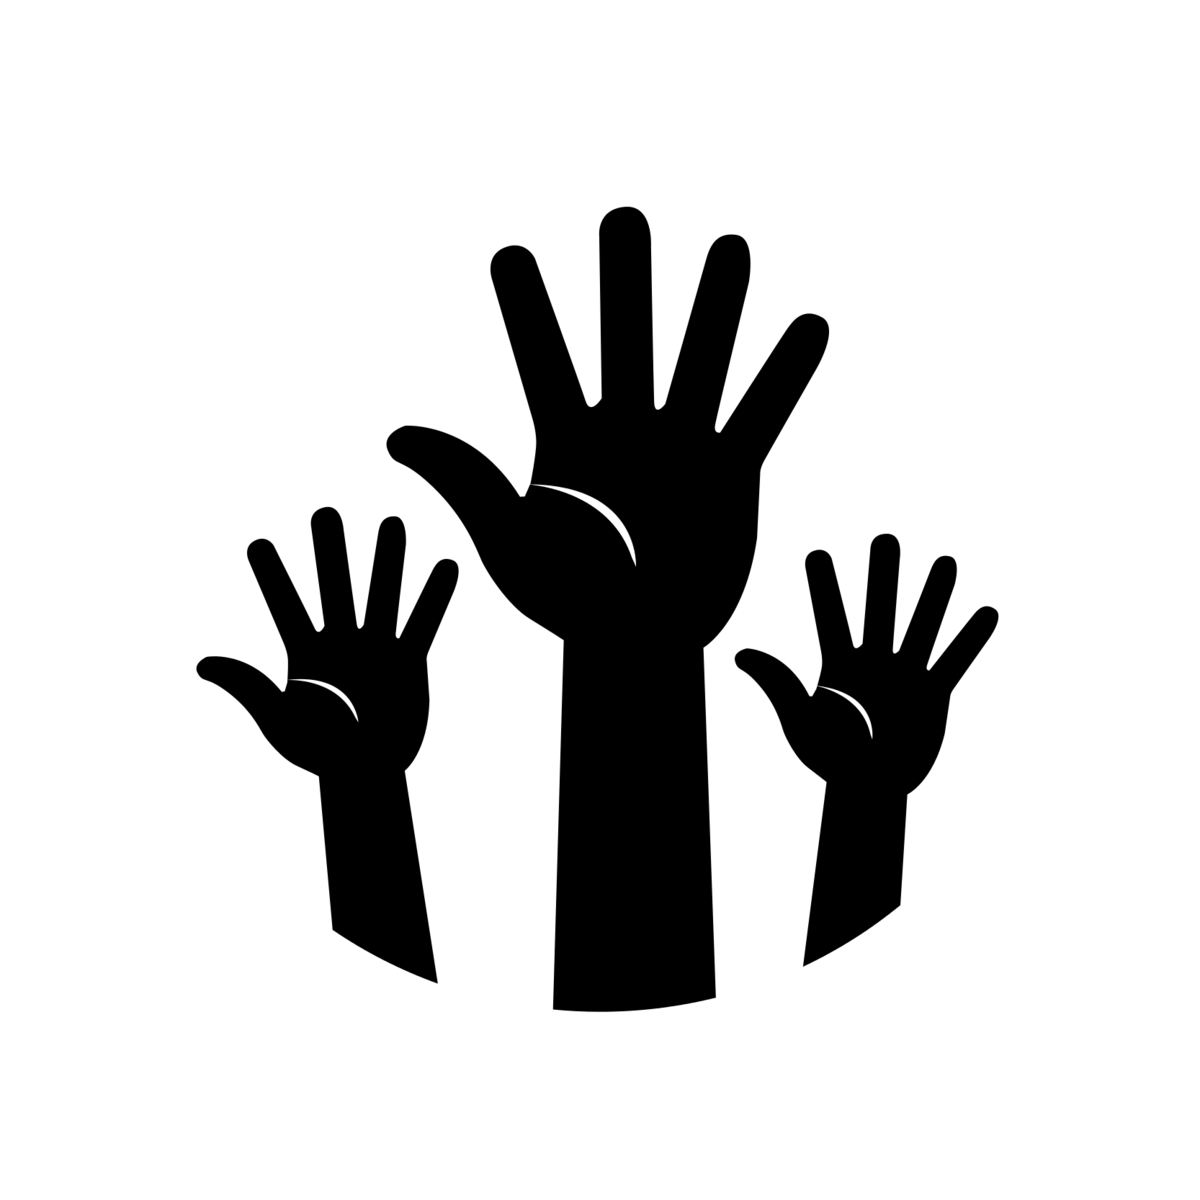
\includegraphics[scale=0.1]{images/hands.png}
}

\only<2->{
\begin{itemize}
  \item Automated machine learning (pipelines, algorithms, hyper-parameters)
  \item Tune robots
  \item Computer vision 
  \item Bioinformatics problems\\(many hard combinatorial or machine learning problems)
  \item AI planning
  \item Compiler optimization
  \item \ldots
\end{itemize}
}

\end{frame}
%----------------------------------------------------------------------
%----------------------------------------------------------------------
\begin{frame}[c]{Quiz}

\centering
\Large
All sessions will include a small quiz:

\textbf{kahoot.it}
\end{frame}
%----------------------------------------------------------------------
%----------------------------------------------------------------------
\begin{frame}[c]{Course Overview}

\begin{itemize}
\item Algorithm Selection
  \begin{itemize}
    \item Portfolios
    \item Algorithm selection for runtime
  \end{itemize}
  \item Design Decisions:\\ Local Search + Evo. Algorithms + Machine Learning 
  \item Empirical evaluation
  \item AAD for ML
  \begin{itemize}
    \item Hyperparameter optimization and Bayesian Optimization 
    \item Neural architecture search (lecture given by Prof. Hutter)
  \end{itemize}
  \item Algorithm configuration 
  \begin{itemize}
    \item Basics 
    \item State of the art 
    \item Best Practices 
  \end{itemize}
  \item Combinations of algorithm selection and configurations
  \item Algorithm control 
  \item Algorithm analysis 
  \item Project announcment and questions for exam 
\end{itemize}

\end{frame}
%----------------------------------------------------------------------
%----------------------------------------------------------------------
% \begin{frame}[c]{Team}
% 
% \begin{columns}[T]
% \column{0.7\textwidth}
% \begin{itemize}
%   \item Frank Hutter
%   \item Head of machine learning lab 
%   \item PhD at the University of British Columbia (Canada)
%   \item Background: Machine learning and combinatorial optimization
% 	\item Expertise in algorithm configuration, algorithm selection, automated machine learning,\ldots
% \end{itemize}
% \column{0.3\textwidth}
% \vspace*{0.7cm}
% 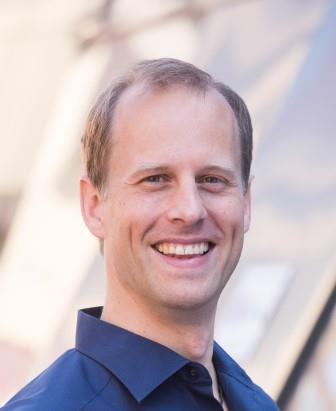
\includegraphics[width=6.7em]{images/team/frank_small}
% 
% \end{columns}
% 
% \end{frame}
%----------------------------------------------------------------------
%----------------------------------------------------------------------
\begin{frame}[c]{Team}

\begin{columns}[T]
\column{0.7\textwidth}
\begin{itemize}
  \item Marius Lindauer
  \item Junior research group lead of automatic algorithm design
  \item PhD at University of Potsdam
  \item Expertise in algorithm configuration, algorithm selection and AutoML
  \item Maintainer of ASlib and AClib
 % \item Background: Hard combinatorial problems (e.g., SAT and ASP)
\end{itemize}
\column{0.3\textwidth}

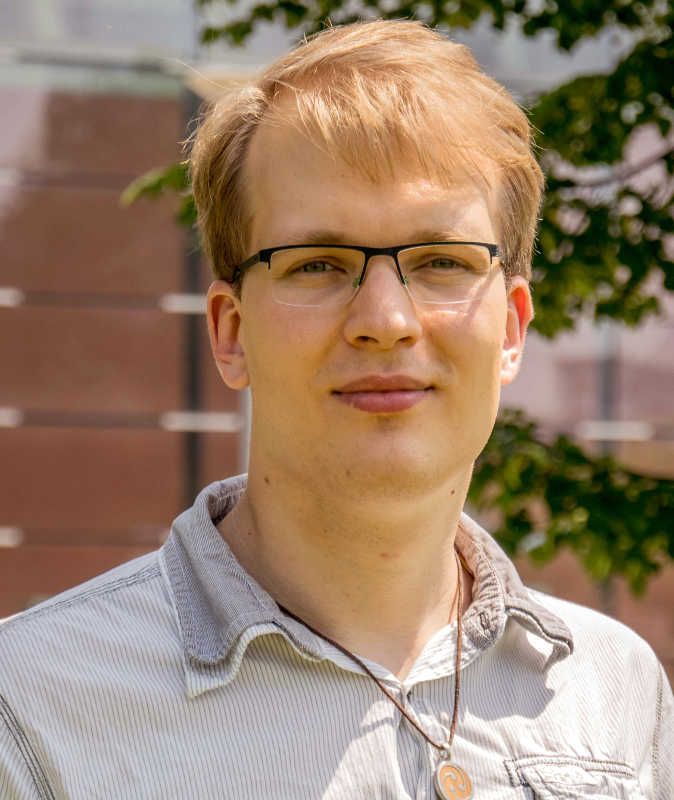
\includegraphics[width=6.7em]{images/team/marius}
\end{columns}

\end{frame}
%----------------------------------------------------------------------
%----------------------------------------------------------------------
\begin{frame}[c]{Team (2)}

\begin{columns}[T]
\column{0.7\textwidth}
\begin{itemize}
  \item Andr\'e Biedenkapp
  \item PhD student
  \item Focus on algorithm control
  \item Responsible for exercises
\end{itemize}
\column{0.3\textwidth}

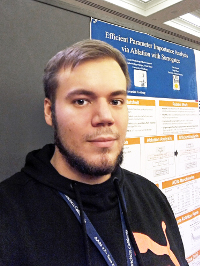
\includegraphics[width=6.7em]{images/team/biedenkapp}
\end{columns}

\end{frame}
%----------------------------------------------------------------------
%----------------------------------------------------------------------
\begin{frame}[c]{Team (Guest Lecturer)}

\begin{columns}[T]
\column{0.7\textwidth}
\begin{itemize}
  \item Frank Hutter
  \item Head of machine learning lab
  \item PhD at the University of British Columbia (Canada)
  \item Background: Machine learning and combinatorial optimization
	\item Expertise in algorithm configuration, algorithm selection, automated machine learning,\ldots
\end{itemize}
\column{0.3\textwidth}
\vspace*{0.7cm}
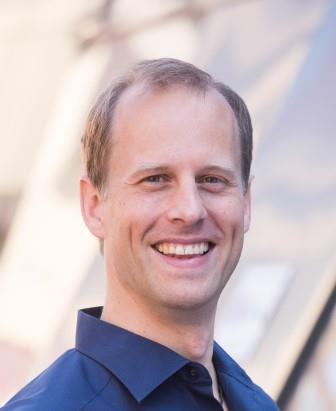
\includegraphics[width=6.7em]{images/team/frank_small}
\end{columns}

\end{frame}
%----------------------------------------------------------------------
%----------------------------------------------------------------------
\begin{frame}[c]{Organization (Lectures)}

\begin{itemize}
  \item $6$ ECTS
  \item Every week at Monday: 14:15 (s.t) - 15:45\\ (Building: 106 Room: SR 00 007)
  \item \emph{Interactive} Lecture 
  \item Course material on our homepage\\
  		{\small \url{ml.informatik.uni-freiburg.de/teaching/ws2018/ml4aad/}}
  \item Slides will be online before the lectures
  \item No video recording!
\end{itemize}


\end{frame}
%-----------------------------------------------------------------------
%----------------------------------------------------------------------
\begin{frame}[c]{Organization (Exercises)}

\begin{itemize}
  \item Every Tuesday at: 12:30 - 14:00\\ (Building: 051 Room: SR 00 006)
  \begin{itemize}
    \item No meeting this week, but first exercise sheet!
  \end{itemize}
  \item Roughly every week new exercise sheet and discussion of last exercise
  \item Most exercises will be practical, i.e., you have to implement something
  \item Team work allowed, max team size: 2! 
  %\item Each exercise will be worth at most $50$ points
  \item Cheating:
  \begin{itemize}
    \item First time cheating: $0$ points for exercise
    \item Second time cheating: failing the course
  \end{itemize}
  \item You have to obtain at least $50\%$ points in the exercises  
  \item Not all assignments will provide the same amount of points
  \item Submit via bitbucket (git)
\end{itemize}

\end{frame}
%-----------------------------------------------------------------------
%----------------------------------------------------------------------
% \begin{frame}[c]{Exceptions (tentative)}
% 
% \begin{itemize}
% 	\item No lectures and exercises during vacations and holidays\\ (1. Nov, 25. Dec, 27. Dec, 01. Jan, 03. Jan)
% 	\item Switching lecture and exercise slot 11. Dec and 13. Dec
% 	\item Last lecture at 05. Feb
% \end{itemize}
% 
% \end{frame}
%-----------------------------------------------------------------------
%----------------------------------------------------------------------
\begin{frame}[c]{Requirements}

\begin{itemize}
  \item Knowledge in Machine Learning (strongly recommended)
  \begin{itemize}
    \item Classification, regression, clustering, decision tree, training-test split, cross validation, deep learning \ldots
  \end{itemize}
  \pause
  \item Basic knowledge in AI 
  \begin{itemize}
    \item decision problems, optimization problems, NP-hard, \ldots 
  \end{itemize}
  \pause
  \item Experience in Python and git 
  \begin{itemize}
    \item nearly all exercises will require that you implement something in~Python and submit the solution to a git repo
  \end{itemize}
\end{itemize}

\end{frame}
%-----------------------------------------------------------------------
%----------------------------------------------------------------------
\begin{frame}[c]{Final Oral Exam}

\begin{itemize}
  \item Implement a larger project (worth $1-2$ weeks fulltime)
	\begin{itemize}
		\item No teamwork!
	\end{itemize}
  \item Exam
	\begin{itemize}
		\item Present the project in the first $15$ minutes\\ (including some questions from us)
		\item Answer questions about further course material in the second $15$ minutes
	\end{itemize}	
\end{itemize}

\end{frame}
%-----------------------------------------------------------------------
%----------------------------------------------------------------------
\begin{frame}[c]{Chances and Risks}

ML4AAD is an advanced lecture and we modify it each time.

\bigskip
\pause

Chances:
\begin{itemize}
  \item All presented topics are close to state-of-the-art;\\there is active research on these topics  
  \item The course will provide a solid background\\ for doing a master project/thesis in our group 
\end{itemize}

\medskip

Risks:
\begin{itemize}
  \item You will find some typos and issues in the slides;\\ please tell us if you find something
  %\item Workload could be very high for you -- we have no experience with the exercises yet
\end{itemize}

\medskip
\pause
$\to$ Give us some feedback and we will improve the course!

\end{frame}
%-----------------------------------------------------------------------
%----------------------------------------------------------------------
\begin{frame}[c]{Introduce yourself!}

\begin{itemize}
  \item Why have you chosen this course?
  \medskip
  \item Background knowledge? (AI, ML, \ldots)
  \medskip 
  \item Experience with such problems?
\end{itemize}

\bigskip
\centering
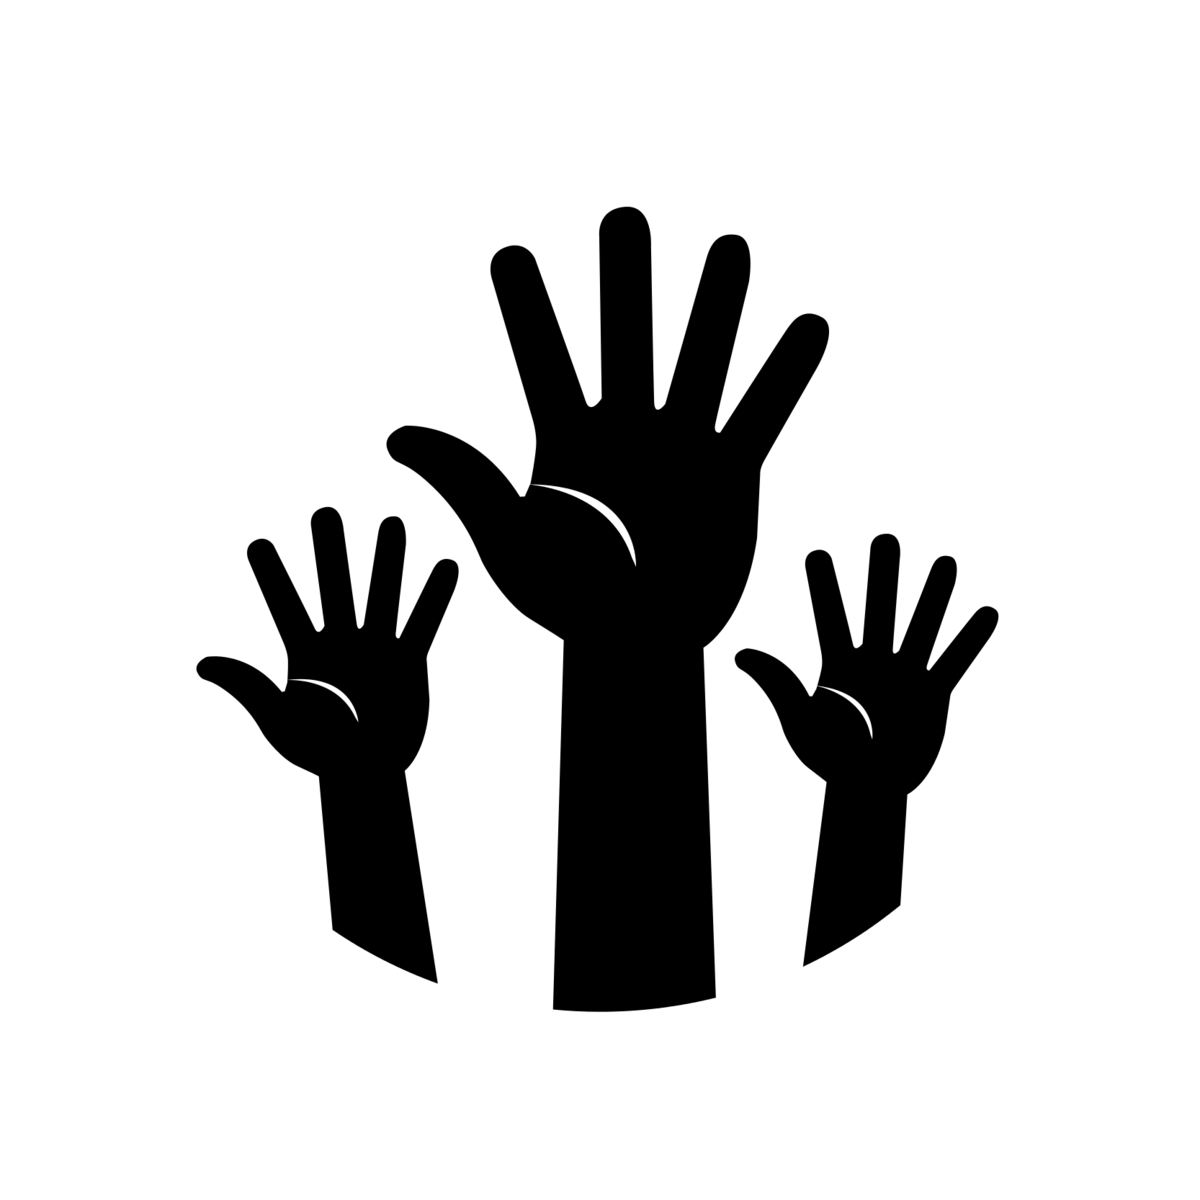
\includegraphics[scale=0.1]{images/hands.png}

\end{frame}
%-----------------------------------------------------------------------
%----------------------------------------------------------------------
% \begin{frame}[c]{Exercise I }
% 
% \begin{block}{Task}
% \begin{enumerate}
% 	\item Identify $2$ (known) algorithms which have tunable parameters and briefly describe these parameters
% 	\item Describe a manual way to tune the parameters and approximate the effort you would need to do this on an example
% 	\item Analyze the runtime complexity of the algorithms
% \end{enumerate}
% \end{block}
% 
% \alert{Submission due 02.11. (23:59 GMT)}\\
% Submit at ILIAS : \url{https://ilias.uni-freiburg.de/goto.php?target=crs_465155&client_id=unifreiburg}
% %Send to: \url{lindauer@cs.uni-freiburg.de}\\
% %with subject: \texttt{[MLOAD Excercise I] $<$your name$>$} 
% 
% \end{frame}
%-----------------------------------------------------------------------
% %----------------------------------------------------------------------
% \begin{frame}[c]{}
% 
% 
% 
% \end{frame}
% %-----------------------------------------------------------------------

